%%%%%%%%%%%%%%%%%%%%%%%%%%%%%%%%%%%%%%%%%

%%%%%%%%%%%%%%%%%%%%%%%%%%%%%%%%%%%%%%%%%

%----------------------------------------------------------------------------------------
%	PACKAGES AND OTHER DOCUMENT CONFIGURATIONS
%----------------------------------------------------------------------------------------

\documentclass[final]{beamer}
\usepackage{bigints}

\usepackage{graphicx} % Required for including images
\graphicspath{{figures/}} % Location of the graphics files
\usepackage{booktabs} % Top and bottom rules for table
\usepackage[font=small,labelfont=bf]{caption} % Required for specifying captions to tables and figures
\usepackage{amsfonts, amsmath, amsthm, amssymb} % For math fonts,  symbols and environments
\usepackage{wrapfig} % Allows wrapping text around tables and figures
\theoremstyle{plain}
\newtheorem{thm}{Theorem}[section]

\newtheorem{prop}[thm]{Proposition}
\newtheorem*{cor}{Corollary}

\theoremstyle{definition}

\newtheorem{conj}{Conjecture}[section]
\newtheorem{exmp}{Example}[section]

\newtheorem{defn}{Definition}[subsection]
\theoremstyle{remark}
\newtheorem*{rem}{Remark}
\usepackage{mathpazo}
\usepackage{mdframed} %Allows text boxes and text background
\usepackage{xcolor}%extends the range of specified colours
\usepackage{float}
\usepackage[scale=1.24]{beamerposter} % Use the beamerposter package for laying out the poster


\usetheme{confposter} % Use the confposter theme supplied with this template
\usepackage{exscale} %allows integrals to be rescaled

\setbeamercolor{block title}{fg=ngreen,bg=white} % Colors of the block titles
\setbeamercolor{block body}{fg=black,bg=white} % Colors of the body of blocks
\setbeamercolor{block alerted title}{fg=white,bg=dblue!70} % Colors of the highlighted block titles
\setbeamercolor{block alerted body}{fg=black,bg=dblue!10} % Colors of the body of highlighted blocks
% Many more colors are available for use in beamerthemeconfposter.sty

%-----------------------------------------------------------
% Define the column widths and overall poster size
% To set effective sepwid, onecolwid and twocolwid values, first choose how many columns you want and how much separation you want between columns
% In this template, the separation width chosen is 0.024 of the paper width and a 4-column layout
% onecolwid should therefore be (1-(# of columns+1)*sepwid)/# of columns e.g. (1-(4+1)*0.024)/4 = 0.22
% Set twocolwid to be (2*onecolwid)+sepwid = 0.464
% Set threecolwid to be (3*onecolwid)+2*sepwid = 0.708

\newlength{\sepwid}
\newlength{\onecolwid}
\newlength{\twocolwid}
\newlength{\threecolwid}
\setlength{\paperwidth}{36in} % A0 width: 46.8in
\setlength{\paperheight}{48in} % A0 height: 33.1in
\setlength{\sepwid}{0.015\paperwidth} % Separation width (white space) between columns
\setlength{\onecolwid}{0.27\paperwidth} % Width of one column
\setlength{\twocolwid}{0.4\paperwidth} % Width of two columns
\setlength{\threecolwid}{0.23\paperwidth} % Width of three columns
\setlength{\topmargin}{-0.5in} % Reduce the top margin size
%-----------------------------------------------------------
\usepackage{environ}
\usepackage{varwidth}
\usepackage{lipsum}
\usepackage{graphicx}  % Required for including images
\usepackage{amssymb}
\usepackage{amsbsy}
\usepackage{mathrsfs}
\usepackage{booktabs} % Top and bottom rules for tables
\usepackage{multicol}
\usepackage[export]{adjustbox}
\usepackage{eso-pic}
\usepackage{mdframed}

%----------------------------------------------------------------------------------------
%	TITLE SECTION 
%----------------------------------------------------------------------------------------
\columnsep=20pt % This is the amount of white space between the columns in the poster
\columnseprule=5pt
\title{Propagation of signals from \vspace{0.5cm} indoor small cells and \vspace{0.5cm} optimization of cell positions} % Poster title

\author{Hayley Wragg} % Author(s)
\def \cosupervisor{Dr. K. Briggs, Dr. M. Fitch}
\def \supervisor{Prof C. J. Budd OBE,  Dr. R. Watson}
\institute{University of Bath} % Institution
 \def \event{Alan Tayler Day, 28th November 2016}
 \def \logo{  
\includegraphics[scale=0.25]{50th-anniversary-logo.png} \hspace{1cm} 
\includegraphics[scale=0.55]{BT.jpg} \hspace{1cm}
 
\includegraphics[scale=1.4]{smithlogo-full.png} \hspace{1cm} 
\includegraphics[scale=0.65]{samba.png} \hspace{1cm} 
\includegraphics[scale=0.4]{imilogo.jpg} }

%----------------------------------------------------------------------------------------

\begin{document}

\usebackgroundtemplate{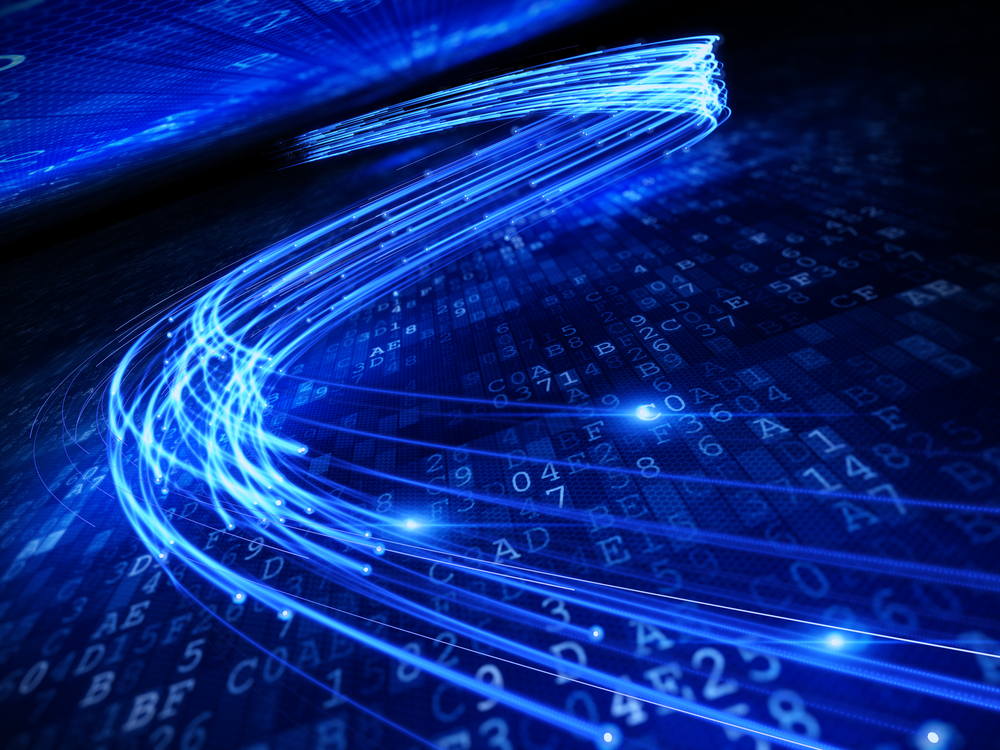
\includegraphics[width=\paperwidth, height=\paperheight]{wifi3}}
\addtobeamertemplate{block end}{}{\vspace*{2ex}} % White space under blocks
\addtobeamertemplate{block alerted end}{}{\vspace*{2ex}} % White space under highlighted (alert) blocks
\addtobeamertemplate{blockNT end}{}{\vspace*{2ex}} % White space under highlighted (alert) blocks

\setlength{\belowcaptionskip}{2ex} % White space under figures
\setlength{\belowdisplayshortskip}{2ex} % White space under equations

\begin{frame}[t] % The whole poster is enclosed in one beamer frame

\begin{columns}[t] % The whole poster consists of three major columns, the second of which is split into two columns twice - the [t] option aligns each column's content to the top

\begin{column}{\sepwid}\end{column} % Empty spacer column

\begin{column}{\onecolwid} % The first column

%---------------------------------------------------------------
% Introduce the team
%---------------------------------------------------------------

  
    \begin{mdframed}[backgroundcolor=white, userdefinedwidth=0.999999\linewidth]
    \centering
    \center
    \usebeamercolor{title in headline}{\color{ForestGreen}\Large{\textbf{\vspace{0.5cm} \\ Who are we? \vspace{0.5cm}}}\\[0.5ex]}
  
    \end{mdframed}
    \vspace{1.5cm}
    
\begin{alertblock}{PhD Student}
\begin{columns} \begin{column}{0.75\linewidth}
\textbf{\insertauthor} \hspace{1cm}
 \\
Previously studied an MMath at the University of Sussex now based at the University of Bath.
\end{column}
\begin{column}{0.25\linewidth}
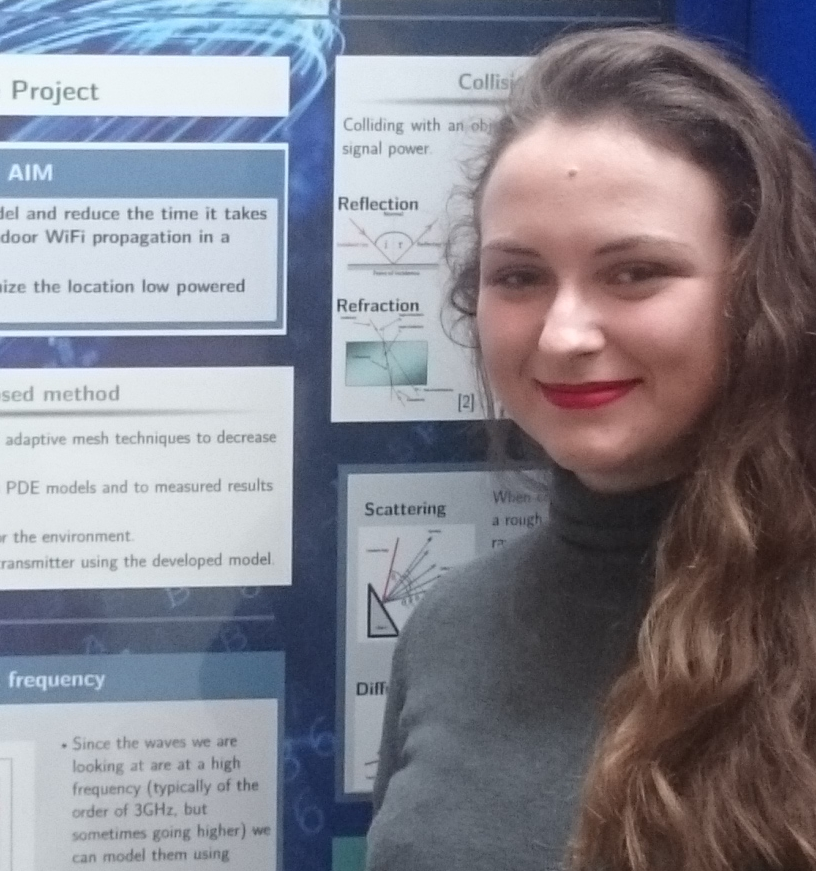
\includegraphics[scale=2]{HWragg.jpg}
\end{column}
\end{columns}
\end{alertblock}

\begin{block}{Supervisors}
\vspace{-2cm}
\begin{columns}
\begin{column}{0.25\linewidth}
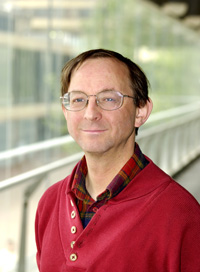
\includegraphics[scale=2.9]{chris-budd.jpg}
\end{column}
\begin{column}{0.75\linewidth}
\textbf{Primary Supervisor: C. Budd}
 \\
Professor of Applied Mathematics at the University of Bath and Professor of Mathematics at the Royal Institution of Great Britain. \\
\end{column}
\end{columns}
\vspace{1cm}
\begin{columns}
\begin{column}{0.75\linewidth}
\textbf{Secondary Supervisor: R. Watson}
 \\
Senior Lecturer in the Dept of Electronic and Electrical Engineering at the University of Bath. \\
\end{column}
\begin{column}{0.25\linewidth}
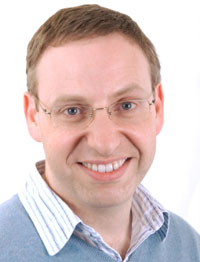
\includegraphics[scale=0.75]{RWatson.jpg}
\end{column}
\end{columns}
\end{block}

\begin{alertblock}{Industrial Supervisors}

\begin{columns}
\begin{column}{0.24\linewidth}
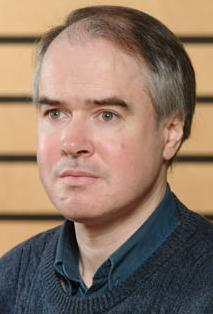
\includegraphics[scale=0.7]{KBriggs.jpg}
\end{column}
\begin{column}{0.74\linewidth}
\textbf{K. Briggs}
 \\
A research mathematician, for BT TSO at Adastral Park. \\
\end{column}
\end{columns}
\begin{columns}
\begin{column}{0.7\linewidth}
\textbf{M. Fitch}
 \\
A research engineer for BT TSO at Adastral Park. \\
\end{column}
\begin{column}{0.24\linewidth}
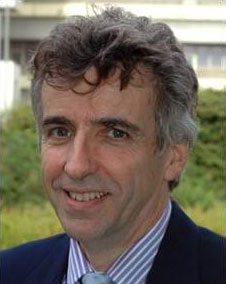
\includegraphics[scale=0.75]{MFitch.jpg}
\end{column}
\end{columns}
\end{alertblock}
 \hspace{0.5in}
 \begin{beamercolorbox}[wd=10in,colsep=0.15cm]{cboxb}
 \end{beamercolorbox}
 \vspace{0.1in}



%------------------------------------------------------------------------------
%		Introduce the location
%--------------------------------------------------------------------------------
    \begin{mdframed}[backgroundcolor=white, userdefinedwidth=0.999999\linewidth]
    \centering
    \center
    \usebeamercolor{title in headline}{\color{ForestGreen}\Large{\vspace{0.5cm} \textbf{Where?} \vspace{0.5cm} }\\[0.5ex]}
    \end{mdframed}
    \vspace{1.5cm}
\begin{block}{Adastral Park}
\begin{columns}
\begin{column}{0.5\linewidth}
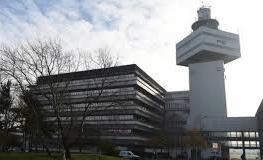
\includegraphics[scale=2.1]{AdastralPark.jpeg} \\ \end{column}
\begin{column}{0.25\linewidth}
Adastral Park is home to the research labs for BT.
\end{column}
\end{columns}
 \vspace{1cm}
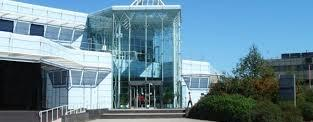
\includegraphics[scale=2.9]{AdastralPark2.jpg}
\end{block}

%---------------------------------------------------------------

\end{column} % End of the first column

\begin{column}{\sepwid}\end{column} % Empty spacer column

\begin{column}{\twocolwid} % Begin a column which is two columns wide (column 2)

%----------------------------------------------------------------------------------------
%	Introduce The Project
%----------------------------------------------------------------------------------------%
\begin{mdframed}[backgroundcolor=white, userdefinedwidth=0.999999\linewidth]
    \centering
    \center
    \usebeamercolor{title in headline}{\color{ForestGreen}\Large{\textbf{\vspace{0.5cm} \\ The Project \vspace{0.5cm}}}\\[0.5ex]}
  
    \end{mdframed}
    \vspace{1.5cm}
\begin{mdframed}[backgroundcolor=white]
\begin{alertblock}{\textbf{AIM}}

\begin{itemize}

\item \textbf{Create an accurate model and reduce the time it takes to simulate indoor-to-indoor WiFi propagation in a domestic environment.}
\item \textbf{Use the model to optimize the location several LTE-femtocells.
}
\end{itemize}
\end{alertblock}
\vspace{-1cm}
\end{mdframed}
\vspace{2cm}



%----------------------------------------------------------------------------------------
\begin{block}{Proposed method}
\vspace{-2cm}
\begin{itemize}
\item Use intelligent algorithms and adaptive mesh techniques to decrease execution time.
\item Compare simulation results to PDE models and to measured results from BT.
\item Develop a stochastic model for the environment.
\item Optimize the location of the transmitter using the developed model.
\end{itemize}
\end{block}
%----------------------------------------------------------------
%		Why is Project required?
%------------------------------------------------------------
 
 \vspace{-2cm}
 \hspace{0.5in}
 \begin{beamercolorbox}[wd=14in,colsep=0.15cm]{cboxb}
 \end{beamercolorbox}
 
\vspace{1cm}
\begin{alertblock}{High volumes of data }
More and more users are requiring high volumes of data. This causes a need for high frequency wave propagation.
\\ 
The high frequency causes a problem with indoor-indoor propagation.
\end{alertblock}

\begin{block}{High frequency}
\vspace{-2cm}
\begin{columns}
\begin{column}{0.45\linewidth}
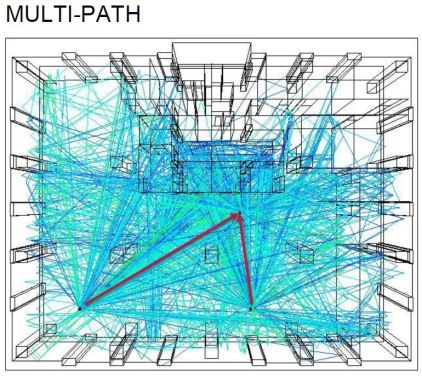
\includegraphics[scale=0.7]{multipath.jpg} \cite{Multipath} 
\end{column}
\begin{column}{0.55\linewidth}
\vspace{-1cm}
\begin{itemize}
\item
Since the waves we are looking at are at a high frequency (typically of the order of 3GHz, but sometimes going higher)  we can model them using ray-tracing.
\item This is very computationally costly to run and requires lots of input information.
\end{itemize}
\end{column}
\end{columns}
\end{block}

\begin{alertblock}{LTE-femtocell}
LTE(Long Term Evolution) femtocells are low-powered base stations for the home designed to allow high speed data transfer
\cite{zyren2007overview, LTEfemtocells}.
\centering
\center
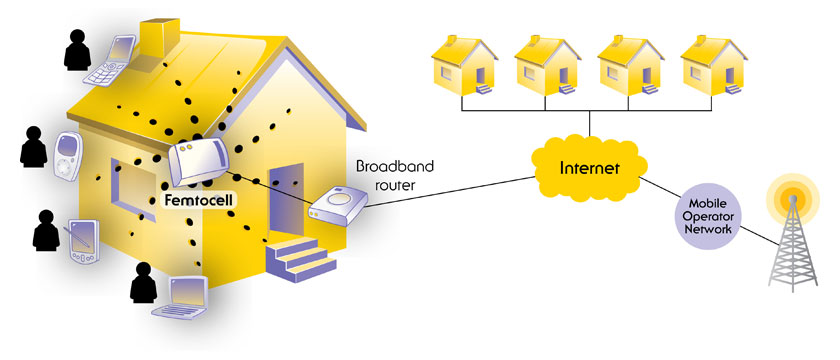
\includegraphics[scale=0.5]{femtocell.jpg} \cite{femtocells} 
\end{alertblock}
%---------------------------------------------------------------------------
%		What is the setting for the Project
%----------------------------------------------------------------
%	Two columns to spilt Image and explanation
\begin{columns}
\begin{column}{0.45\linewidth}

\begin{block}{Domestic Environment}
\vspace{-1cm}
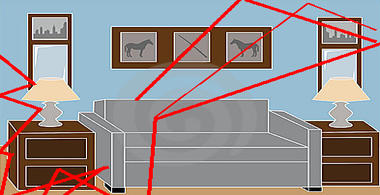
\includegraphics[scale=5.2]{livingroom.jpg} 
\end{block}

\end{column}
\begin{column}{0.01\linewidth}

\end{column}
\begin{column}{0.45\linewidth}
\vspace{-1.25cm}
\begin{mdframed}[backgroundcolor=white, userdefinedwidth=0.999999\linewidth]
\vspace{0.5cm}
\begin{itemize}
\item A domestic environment is very cluttered, which reduces the number of Line of Sight Paths.
\item Each collision results in the wave having a combination of reflections, diffractions, and refractions. 
\end{itemize}
\vspace{0.5cm}
\end{mdframed}

\end{column}
\end{columns}

\end{column} % End of the second column

\begin{column}{\sepwid}\end{column} % Empty spacer column
\begin{column}{\sepwid}\end{column} % Empty spacer column
\begin{column}{\threecolwid} % The third column


%----------------------------------------------------------------------------------------
%	Brief of Collsions with objects
%-------%---------------------------------------------------------------


\begin{block}{Collisions}
\vspace{-1.5cm}

When a wave collides with an object the collision causes a loss in signal power. 
\vspace{0.5cm}
\begin{columns}
\begin{column}{0.5\linewidth}
\textbf{Reflection} \\
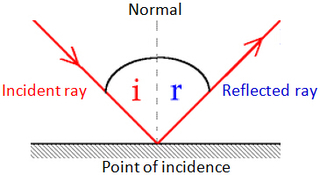
\includegraphics[scale=1]{Reflection.jpg} \cite{Reflection}
\end{column}
\begin{column}{0.5\linewidth}
 \\
After colliding with an object at some angle of incidence $i$ a ray is then reflected at an angle of reflection $r$.
\end{column}
\end{columns}
\begin{columns}
\begin{column}{0.5\linewidth}
\textbf{Refraction} \\
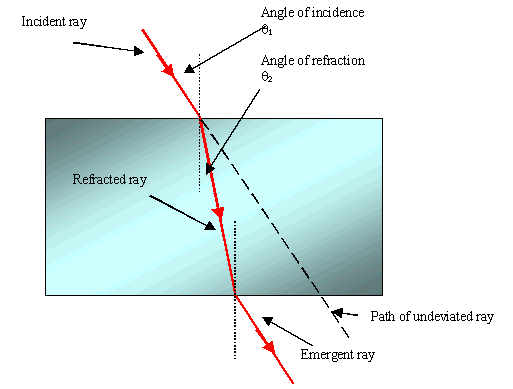
\includegraphics[scale=0.5]{Refraction.png} 
\cite{Refraction} 
\end{column}
\begin{column}{0.5\linewidth}
When a ray travels through an object it is refracted slightly towards the normal.
\end{column}
\end{columns}
\end{block}

\begin{mdframed}[backgroundcolor=jblue!15, linecolor=jblue!70,
  linewidth=20pt,
  topline=true,
  rightline=true,
  leftline=true, bottomline=true, userdefinedwidth=0.999999999999999\linewidth]
  \begin{columns}
  \begin{column}{0.01\linewidth}
  \end{column}
  \begin{column}{0.445\linewidth}
\textbf{Scattering} \\
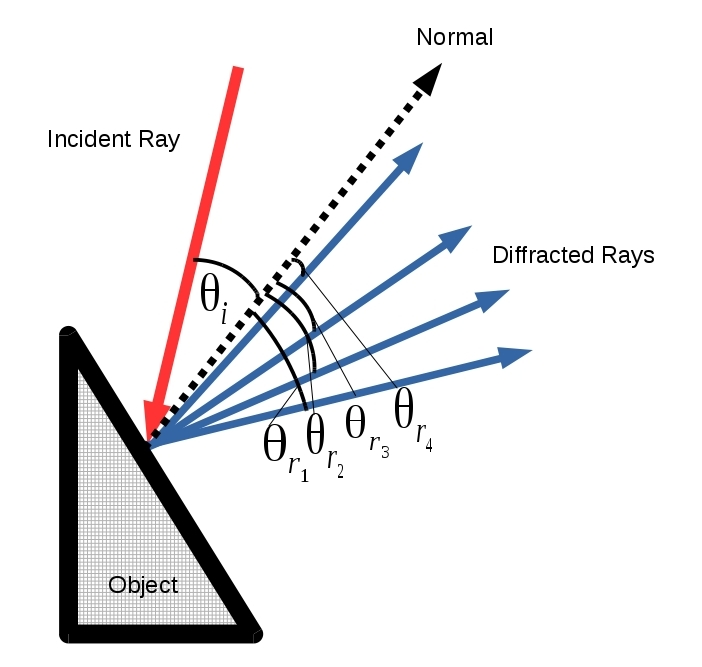
\includegraphics[scale=0.47]{Scattering.jpg} 
\\   
\end{column}

\begin{column}{0.53\linewidth}
When colliding with a rough surface a ray can scatter. This can be unpredictable and can be computationally costly to simulate. \cite{Antennas2007}
 \end{column}
 \end{columns}
 \vspace{1cm}
 \begin{columns}
 \begin{column}{0.01\linewidth}
  \end{column}
\begin{column}{0.445\linewidth}
\textbf{Diffraction} \\
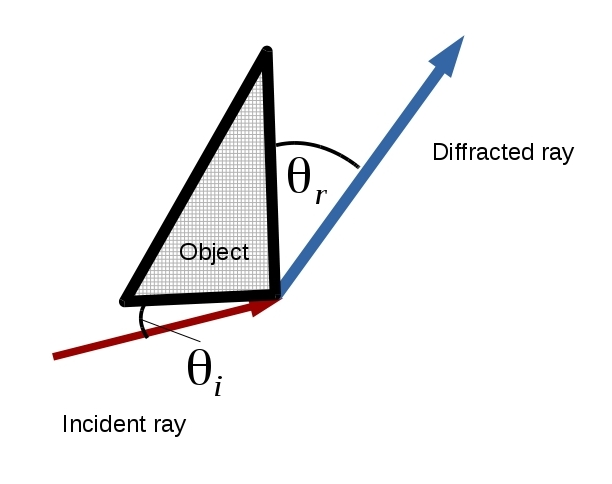
\includegraphics[scale=0.53]{Diffraction.jpg}
\end{column}
\begin{column}{0.53\linewidth}
Collision with the corner of an object this causes the ray to diffract which is also difficult to predict.
\end{column}
\end{columns}
\end{mdframed}



%----------------------------------------------------------------------------------------
%----------------------------------------------------------------------------------------

-------------------------------------
%	Weak Solution
%----------------------------------------------------------------------------------------






%----------------------------------------------------------------------------------------
%----------------------------------------------------------------------------------------
%	REFERENCES
%----------------------------------------------------------------------------------------
\setbeamercolor{block alerted title}{fg=black,bg=CadetBlue} % Change the alert block title colors
\setbeamercolor{block alerted body}{fg=black,bg=white} % Change the alert block body colors

\begin{alertblock}{References}

\nocite{*} % Insert publications even if they are not cited in the poster
\tiny{\scalebox {.2}{\bibliographystyle{unsrt}} \bibliography{posterattempt1.bib}
 \vspace{0.4in}}

\end{alertblock}
%----------------------------------------------------------------------------------------
%-------------------------
%	CONTACT INFORMATION
%--------------------------------------------------------------------------------------


\begin{alertblock}{Contact Information} \small

\begin{itemize}
%\item Web: \href{https://uk.linkedin.com/in/hw236}{https://uk.linkedin.com/in/hw236}
\item Email: \href{mailto:hw454@bath.ac.uk}{hw454@bath.ac.uk}

\end{itemize}

\end{alertblock}

%----------------------------------------------------------------------------------------
%	ACKNOWLEDGEMENTS
%----------------------------------------------------------------------------------------

% \setbeamercolor{block title}{fg=red,bg=white} % Change the block title color

% \begin{block}{Acknowledgements}

% \small{\rmfamily{Dr Anotida Madvamuse}}
% \\
% \small{\rmfamily{Dr ChandrasekharVenkataraman  }}

% \end{block}

%---------------------------------------------------------------

\end{column} % End of the third column

\end{columns} % End of all the columns in the poster

\end{frame} % End of the enclosing frame

\end{document}
